\documentclass{article}

% if you need to pass options to natbib, use, e.g.:
%     \PassOptionsToPackage{numbers, compress}{natbib}
% before loading neurips_2026

% The authors should use one of these tracks.
% Before accepting by the NeurIPS conference, select one of the options below.
% 0. "default" for submission
\usepackage{neurips_2026}
% the "default" option is equal to the "main" option, which is used for the Main Track with double-blind reviewing.
% 1. "main" option is used for the Main Track
%  \usepackage[main]{neurips_2026}
% 2. "position" option is used for the Position Paper Track
%  \usepackage[position]{neurips_2026}
% 3. "eandd" option is used for the Evaluations & Datasets Track
 % \usepackage[eandd]{neurips_2026}
 % if you need to opt-in for a single-blind submission in the E&D track:
 %\usepackage[eandd, nonanonymous]{neurips_2026}
% 4. "creativeai" option is used for the Creative AI Track
%  \usepackage[creativeai]{neurips_2026}
% 5. "sglblindworkshop" option is used for the Workshop with single-blind reviewing
 % \usepackage[sglblindworkshop]{neurips_2026}
% 6. "dblblindworkshop" option is used for the Workshop with double-blind reviewing
%  \usepackage[dblblindworkshop]{neurips_2026}

% After being accepted, the authors should add "final" behind the track to compile a camera-ready version.
% 1. Main Track
 % \usepackage[main, final]{neurips_2026}
% 2. Position Paper Track
%  \usepackage[position, final]{neurips_2026}
% 3. Evaluations & Datasets Track
 % \usepackage[eandd, final]{neurips_2026}
% 4. Creative AI Track
%  \usepackage[creativeai, final]{neurips_2026}
% 5. Workshop with single-blind reviewing
%  \usepackage[sglblindworkshop, final]{neurips_2026}
% 6. Workshop with double-blind reviewing
%  \usepackage[dblblindworkshop, final]{neurips_2026}
% Note. For the workshop paper template, both \title{} and \workshoptitle{} are required, with the former indicating the paper title shown in the title and the latter indicating the workshop title displayed in the footnote.
% For workshops (5., 6.), the authors should add the name of the workshop, "\workshoptitle" command is used to set the workshop title.
% \workshoptitle{WORKSHOP TITLE}

% "preprint" option is used for arXiv or other preprint submissions
 % \usepackage[preprint]{neurips_2026}

% to avoid loading the natbib package, add option nonatbib:
%    \usepackage[nonatbib]{neurips_2026}

\usepackage[utf8]{inputenc} % allow utf-8 input
\usepackage[T1]{fontenc}    % use 8-bit T1 fonts
\usepackage{hyperref}       % hyperlinks
\usepackage{url}            % simple URL typesetting
\usepackage{amsmath}        % for mathematical environments
\usepackage{array}          % column-specific table formatting
\usepackage{booktabs}       % professional-quality tables
\usepackage{graphicx}       % resize oversized table entries
\usepackage{longtable}      % multi-page tables
\usepackage{xltabular}      % longtable with text-width columns
\usepackage{amsfonts}       % blackboard math symbols
\usepackage{nicefrac}       % compact symbols for 1/2, etc.
\usepackage{microtype}      % microtypography
\usepackage[table]{xcolor} % colors, including table cells
\usepackage{cleveref}
\usepackage{subcaption}
\usepackage{todonotes}

\newcommand{\konrad}[1]{\todo[inline,color=green!40]{Konrad: #1}}

% Note. For the workshop paper template, both \title{} and \workshoptitle{} are required, with the former indicating the paper title shown in the title and the latter indicating the workshop title displayed in the footnote. 
\title{A Continuous Detour to Ramsey Graphs: Frank-Wolfe for Non-Monotone Supermodular Objectives}


% The \author macro works with any number of authors. There are two commands
% used to separate the names and addresses of multiple authors: \And and \AND.
%
% Using \And between authors leaves it to LaTeX to determine where to break the
% lines. Using \AND forces a line break at that point. So, if LaTeX puts 3 of 4
% authors names on the first line, and the last on the second line, try using
% \AND instead of \And before the third author name.


\author{%
  David S.~Hippocampus\thanks{Use footnote for providing further information
    about author (webpage, alternative address)---\emph{not} for acknowledging
    funding agencies.} \\
  Department of Computer Science\\
  Cranberry-Lemon University\\
  Pittsburgh, PA 15213 \\
  \texttt{hippo@cs.cranberry-lemon.edu} \\
  % examples of more authors
  % \And
  % Coauthor \\
  % Affiliation \\
  % Address \\
  % \texttt{email} \\
  % \AND
  % Coauthor \\
  % Affiliation \\
  % Address \\
  % \texttt{email} \\
  % \And
  % Coauthor \\
  % Affiliation \\
  % Address \\
  % \texttt{email} \\
  % \And
  % Coauthor \\
  % Affiliation \\
  % Address \\
  % \texttt{email} \\
}


\begin{document}


\maketitle


\begin{abstract}
    Establishing Ramsey number lower bounds constitutes a well-studied class of hard combinatorial feasibility problems. Known lower-bound witnesses have accumulated over decades through problem-specific discrete heuristics, with several key values remaining out of reach for generic methods. We replace direct graph-space search by continuous optimization on a hypercube relaxation, with binary graph structure retained through the oracle, rounding, and verification. Casting the construction problem as minimization of a pseudo-Boolean polynomial violation count turns satisfiability into optimization; relaxing the binary constraints to the unit hypercube then yields a smooth multilinear objective.

    Frank-Wolfe performs surprisingly well on this relaxation, even though the objective is non-monotone supermodular and only stationarity guarantees apply. At each step its hypercube linear minimization oracle returns a binary vertex, anchoring iterates to concrete candidates. A conditional-expectations rounding converts the fractional iterate to a binary candidate without increasing the violation count.

    This pipeline recovers a significant portion of the known lower-bound table, most notably finding $42$-vertex graphs certifying $R(5,5) \geq 43$. Recent LLM-driven evolutionary search using AlphaEvolve (Nagda et al., 2026) reports new off-diagonal lower bounds but does not report this long-standing benchmark.
\end{abstract}



\section{Introduction}

Hard combinatorial feasibility problems can often be reformulated as smooth optimization: penalize the violations in the objective and relax binary variables to the unit hypercube, yielding a differentiable problem accessible to first-order methods. For structured objective classes this yields tight theory --- Continuous Greedy, for example, attains a $(1-1/e)$ approximation for monotone submodular maximization under matroid constraints by linear optimization over the feasible polytope~\cite{vondrak2008optimal,calinescu2011maximizing}. For non-monotone supermodular objectives no comparable $(1-1/e)$-type guarantee is known, and the underlying combinatorial problems are typically NP-hard, so continuous reformulation does not rescue global optimality. The relevant question is therefore empirical: do first-order methods find useful discrete witnesses in practice? Generic nonconvex Frank-Wolfe~\cite{braun2022conditional} gives only stationarity guarantees, so no theorem-level argument forces it to. We use it as a search heuristic, motivated separately by an algorithmic property: on the hypercube its linear minimization oracle returns a binary vertex at every step, anchoring each iterate to a concrete candidate discrete witness. Ramsey lower-bound search is a natural test case: it is well studied, has a long record of specialized constructive methods, and every candidate graph can be checked exactly.

The Ramsey number $R(r,s)$ is the critical graph order at which every graph must contain either a clique of size $r$ or an independent set of size $s$. Certifying $R(r,s) > n$ requires producing a graph on $n$ vertices with clique number strictly less than $r$ and independence number strictly less than $s$. Several key values have resisted decades of effort; for example, the best current bounds for $R(5,5)$ are $43 \leq R(5,5) \leq 46$. Prior constructive lower-bound approaches, including local search heuristics such as simulated annealing and tabu search, extensions of known Ramsey graphs, constructions restricted to algebraic families such as circulant or Cayley graphs, and recent LLM-generated search programs, have largely operated in discrete search spaces.

Progress in Ramsey lower-bound search takes three distinct forms. The most direct is improving a known lower bound by exhibiting a witness on more vertices than any prior construction. Less direct but still informative is finding new extremal witnesses at the same order: classifications of frontier Ramsey graphs remain far from complete, and each new construction enriches the structural picture. Recovering known witnesses through a markedly different method also matters: it tests whether the method reaches the relevant part of the search space without being tailored to known constructions, and provides computational evidence about how thoroughly that space has been explored.

We tie the continuous-optimization viewpoint above to the Ramsey construction problem by turning Ramsey satisfiability into optimization. The hard Ramsey constraints are moved into a pseudo-Boolean polynomial violation objective on the edge variables. This first step replaces a discrete feasibility question by minimization of a violation count; relaxing the edge variables from binary to the unit interval then turns it into a differentiable multilinear optimization problem on a convex domain. The LMO on the hypercube takes the simplest possible form: at each iterate, it returns the binary graph determined by the coordinatewise sign of the gradient, so each Frank-Wolfe step pulls the iterate toward a candidate discrete witness. The raw violation objective is non-monotone supermodular: the clique and independent-set terms are both supermodular but have opposite monotonicities. For search, we optimize a log-barrier surrogate of this raw objective, which sharpens gradient signal for vertex sets whose monochromatic probability is already close to one and empirically outperforms direct optimization of the raw violation count as a search loss. Candidates obtained from this surrogate are still rounded and certified against the original Ramsey constraints. The raw objective itself admits a combinatorial reading: with each edge weight interpreted as the probability that the corresponding edge appears, its value is exactly the expected number of cliques of size $r$ and independent sets of size $s$ in the resulting random graph. Conditional-expectations rounding derandomizes this expectation by fixing edges one at a time, extracting a binary candidate without increasing the violation objective --- the algorithmic form of Erd\H{o}s's probabilistic-method existence argument for Ramsey lower bounds~\cite{erdos1947remarks}.

\paragraph{Contributions.}
\begin{enumerate}
    \item We develop a projection-free Frank-Wolfe pipeline for the multilinear hypercube relaxation of the Ramsey violation objective --- closed-form LMO, stochastic clique batching, and conditional-expectations rounding with exact verification --- run without algebraic restrictions on the graph structure.
    \item We show empirically that this pipeline recovers a broad set of known Ramsey lower-bound witnesses, including repeated recovery of $42$-vertex graphs certifying $R(5,5)>42$, a long-standing frontier construction not reported by the recent AlphaEvolve Ramsey search.
\end{enumerate}

\paragraph{Related Literature.}
Frank-Wolfe methods are projection-free first-order algorithms for smooth optimization over convex sets with efficient LMOs~\cite{frank1956algorithm,jaggi2013revisiting,braun2022conditional}. Variants such as away-step and pairwise Frank-Wolfe modify the active-set dynamics and can obtain stronger convergence guarantees under additional convexity and geometric assumptions~\cite{lacostejulien2015global}. Our use is closest to the basic nonconvex conditional-gradient viewpoint: over the edge hypercube, the LMO is separable and returns a binary graph, while generic theory supplies guarantees on stationarity or the Frank-Wolfe gap rather than approximation or certificate guarantees.

Continuous Greedy is the canonical multilinear-extension method for submodular maximization. Vondr{\'a}k introduced the continuous-greedy framework, with submodular welfare as the headline application~\cite{vondrak2008optimal}, and Calinescu, Chekuri, P{\'a}l, and Vondr{\'a}k developed the multilinear-extension approach for monotone submodular maximization under matroid constraints; continuous greedy plus pipage rounding yields a $(1-1/e)$ approximation~\cite{calinescu2011maximizing}. Pipage rounding and contention-resolution schemes are central fractional-to-integral tools in this line of work~\cite{ageev2004pipage,chekuri2011contention}. Our extraction step is different, using conditional expectations over the independent-edge model on the full hypercube. The connection is therefore methodological rather than theorem-level: our pipeline uses the same multilinear relaxation and the same vertex-returning linear oracle, and applies a fractional-to-binary rounding step, but the raw Ramsey objective is a non-monotone supermodular violation-minimization objective rather than a monotone submodular utility.

Non-monotone submodular maximization has its own algorithmic literature, including randomized and DoubleGreedy-style algorithms for unconstrained nonnegative objectives~\cite{feige2011maximizing,buchbinder2015tight}. For the box-constrained setting that the Ramsey objective enters after sign-flipping and shifting, continuous-greedy-type methods are the closer comparators. Feldman, Naor, and Schwartz introduced a unified continuous-greedy framework for nonnegative non-monotone submodular maximization over down-monotone polytopes~\cite{feldman2011unified}. Bian et al.\ study continuous submodular and diminishing-returns (DR)-submodular maximization; their monotone result has a Frank-Wolfe/Continuous-Greedy flavor, while their non-monotone box-constrained method is DoubleGreedy-style and coordinatewise rather than LMO-driven~\cite{bian2017guaranteed}. Mokhtari, Hassani, and Karbasi develop stochastic conditional-gradient methods, including non-monotone stochastic continuous greedy for DR-submodular maximization~\cite{mokhtari2020stochastic}. These methods provide approximation-ratio guarantees on objective value, whereas Ramsey lower-bound construction needs an exact zero-violation witness ($M=0$), which a constant-factor approximation of the shifted nonnegative utility $C-M$ does not deliver. Our pipeline runs vanilla Frank-Wolfe over the full edge hypercube --- combining fractional iterates with binary oracle outputs --- and applies conditional-expectations rounding and exhaustive verification to the raw violation count.

We defer the detailed Ramsey chronology, bound table, and comparison with prior constructive methods to \cref{sec:problem}.

% -----------------------------------------------------------------------
% Draft material below: Konrad's original introduction, kept for reference
% -----------------------------------------------------------------------
\iffalse
\newpage

Discrete optimization problems in extremal combinatorics often have a useful asymmetry: finding an optimum may be difficult, but checking a proposed witness can be exact and cheap relative to the search. Ramsey lower bounds are a canonical example. To prove $R(r,s)>n$, it suffices to exhibit a graph on $n$ vertices with no clique of size $r$ and no independent set of size $s$, or equivalently a two-coloring of the edges of the complete graph $K_n$ with no forbidden monochromatic clique. This makes Ramsey search a useful benchmark for optimization heuristics: the search space has size $2^{\binom{n}{2}}$, the landscape is highly nonconvex and high-order, and every successful output is independently verifiable.

Recent computational progress in extremal combinatorics has relied on a broad spectrum of ideas, including classical local search, cross-entropy methods, neural constructions, and LLM-assisted heuristic discovery \cite{Rubinstein2004,wagner2021constructions,nagda2026reinforcedgenerationcombinatorialstructures}. These methods often exploit restrictions of the search space, such as algebraic, circulant, vertex-transitive, Cayley, or vertex-by-vertex constructions, which can reduce the number of effective variables from quadratic in $n$ to nearly linear. Such restrictions are powerful, but they raise the usual question of whether the imposed structure excludes the relevant optima. The complementary approach we study here is to keep the full edge-variable search space and relax the discrete problem into a differentiable one.

Our guiding question is therefore not whether continuous optimization replaces specialized Ramsey search, but whether a standard first-order method can serve as a broadly useful discrete-optimization heuristic on this hard, exactly certified task. Frank-Wolfe methods are attractive in this role because their linear minimization oracle over a hypercube or product of simplices returns an extreme point. Each update is projection-free, inexpensive once gradients are available, and geometrically biased toward the discrete colorings that ultimately need to be certified \cite{frank1956algorithm,braun2022conditional}. This is the main narrative of the paper: Ramsey search exposes a setting where conditional gradients are not merely a way to solve a relaxation, but a mechanism for steering a continuous iterate toward useful combinatorial witnesses.

We structure the paper as follows. \cref{eq:no-monochromatic-cliques} turns Ramsey search into a pseudo-Boolean polynomial objective; the continuous relaxation gives a probabilistic interpretation as the expected number of forbidden cliques; the surrogate losses reshape the gradients around near-violations; Frank-Wolfe supplies a simple projection-free update; stochastic clique batching makes the method scalable; and conditional expectation plus exhaustive checking turns relaxed candidates into certified graphs. We refer to \cite{morris2026recentresultsramseytheory} for recent Ramsey-theoretic background.

\paragraph{Contributions.}
\begin{itemize}
  \item We frame Ramsey lower-bound search as a testbed for Frank-Wolfe type methods as heuristics for hard discrete and combinatorial optimization.
  \item We connect the classical satisfiability view of Ramsey witnesses to a pseudo-Boolean clique-counting objective and its natural probabilistic continuous relaxation.
  \item We use clique-wise surrogate losses, including a log-barrier variant, to emphasize potentially monochromatic cliques while preserving the structure of the original objective.
  \item We describe a projection-free conditional-gradient pipeline with stochastic clique batching, deterministic conditional-expectation extraction, and exact verification.
  \item Empirically, the method recovers strong diagonal and near-diagonal witnesses, including repeated recovery of $42$-vertex colorings certifying $R(5,5)>42$.
\end{itemize}
\fi


\section{The Problem: Constructing Ramsey Graphs}\label{sec:problem}

An $n$-vertex graph $G$ is an $(r,s,n)$-Ramsey graph if it contains no clique of size $r$ and no independent set of size $s$, i.e., $\omega(G) < r$ and $\alpha(G) < s$. The Ramsey number $R(r,s)$ is the least $n$ for which no such graph exists; the case $r = s$ is called diagonal and $r \neq s$ off-diagonal. Proving the lower bound $R(r,s) > n$ amounts to exhibiting a single $(r,s,n)$-Ramsey graph, while the upper bound $R(r,s) \leq n$ requires ruling out all such graphs at order $n$; we address the lower-bound construction side. Verifying a candidate $G$ reduces to clique-existence tests; for fixed $r,s$ this is polynomial in $n$ by brute enumeration and well-handled in practice by solvers such as Cliquer~\cite{niskanen2003cliquer}. The bottleneck is search: the graph spaces is exponential in $n$, even after quotiening by isomorphism, which quickly does not make exhaustive construction a viable approach.

% Previous standalone asymptotic paragraph (compressed into the opening sentence
% below). Kept here for reference in case we want to restore the longer form.
\iffalse
The asymptotic theory of Ramsey numbers has long-standing exponential gaps. On the diagonal, the original Erdős-Szekeres bound~\cite{erdosszekeres1935} gives $R(k,k) = O(4^k / \sqrt{k})$, while the probabilistic argument of Erdős~\cite{erdos1947remarks} gives $R(k,k) \geq 2^{k/2}$. The first exponential improvement on the upper bound, $R(k,k) \leq (4-\epsilon)^k$ for some $\epsilon > 0$, was obtained only recently by Campos, Griffiths, Morris, and Sahasrabudhe~\cite{campos2023exponential} and subsequently refined to $R(k,k) \leq 3.8^k$ by Gupta, Ndiaye, Norin, and Wei~\cite{gupta2024optimizing}; the gap between the two exponents remains. Off-diagonal cases admit polynomial scaling in the second parameter: $R(3,k) = \Theta(k^2/\log k)$~\cite{aks1980,kim1995r3k}, with the lower-bound constant recently tightened to $(1/2 + o(1)) k^2/\log k$ by Hefty, Horn, King, and Pfender~\cite{hefty2025r3k}; for $R(4,k)$, Mattheus and Verstraete~\cite{mattheus2024r4t} established the asymptotic exponent $R(4,k) = k^{3+o(1)}$.
\fi

Asymptotically, $2^{k/2} \leq R(k,k) \leq (4-\epsilon)^k$~\cite{erdos1947remarks,campos2023exponential,gupta2024optimizing}, while $R(3,k) = \Theta(k^2/\log k)$~\cite{aks1980,kim1995r3k} (recently tightened by Hefty, Horn, King, and Pfender~\cite{hefty2025r3k}; see also Mattheus-Verstraete~\cite{mattheus2024r4t} for $R(4,k)$, and Morris~\cite{morris2026recentresultsramseytheory} for a survey of recent progress). The concrete table is far sparser; Radziszowski's dynamic survey and McKay's graph database collect known exact values, bounds, and witness graphs~\cite{radziszowski2026smallramsey,mckayramseydata}. Greenwood and Gleason's $R(3,3) = 6$ and $R(4,4) = 18$~\cite{greenwood1955combinatorial} have classical proofs; the next exact value, McKay and Radziszowski's $R(4,5) = 25$~\cite{mckayradziszowski1995r45}, requires substantial computation. Several nearby cases remain open, including $40 \leq R(3,10) \leq 41$ and the flagship diagonal gap $43 \leq R(5,5) \leq 46$: the lower bound comes from Exoo's 42-vertex construction~\cite{exoo1989lower}, while the upper bound has moved through a sequence of computer-assisted improvements over more than three decades~\cite{mckayradziszowski1997subgraph,angeltveitmckay2018r55leq48} to the current Angeltveit-McKay bound~\cite{angeltveit2026r55leq46}.

Exact small-value progress combines lower-bound witness construction with upper-bound exclusion, both supported by certifying or exhaustive computation. The techniques include vertex-by-vertex extension and gluing~\cite{mckayradziszowski1995r45,angeltveitmckay2018r55leq48}, subgraph-counting identities~\cite{mckayradziszowski1997subgraph}, LP pruning~\cite{angeltveit2026r55leq46}, SAT with abstraction and symmetry breaking~\cite{codish2016r433}, SAT modulo symmetries~\cite{kirchwegerszeider2024}, and flag-algebra and SDP techniques in adjacent Ramsey settings~\cite{razborov2007flag,lidickypfender2021sdp}. At small instance sizes, isomorph-free generation, extension searches, and SAT enumeration can produce explicit lower-bound witnesses or exhaustively enumerate them, with the latter supporting upper-bound exclusion at the next order. Beyond that regime, constructive progress on lower bounds has largely relied on heuristic search.

Heuristic constructive search uses structural priors, local objectives, stochastic search, or learned heuristics. Circulant and cyclic restrictions reduce the variable count from $\Theta(n^2)$ to $O(n)$~\cite{kalbfleisch1965,exootatarevic2015}; broader algebraic priors include Paley graphs, Cayley graphs, and other vertex-transitive families~\cite{mathon1987}. Local search uses recoloring moves over the chosen representation --- single edges, circulant distances, or block-circulant entries --- with simulated annealing, tabu search, or adaptive bad-subgraph objectives~\cite{piwakowski1996tabu,exootatarevic2015}. Stochastic methods include the cross-entropy method~\cite{Rubinstein2004} and neural or reinforcement-learning approaches in extremal combinatorics~\cite{wagner2021constructions}; Ramsey-specific follow-ups have produced mixed results, with positive constructions from GNN generation~\cite{ghoselevizhang2022} and bounds for non-classical Ramsey targets via reinforcement learning~\cite{ghebleh2024}, alongside a documented negative deep-RL result on classical small Ramsey instances~\cite{berghaus2025}. Recent LLM-driven evolutionary search~\cite{nagda2026reinforcedgenerationcombinatorialstructures}, building on AlphaEvolve~\cite{novikov2025alphaevolve} and Funsearch~\cite{romeraparedes2024funsearch}, produces new off-diagonal bounds. Successful constructive searches at larger off-diagonal cases typically exploit such structure, though complete small-case catalogues contain many low-symmetry graphs.

The $R(5,5,42)$ case has become a challenging heuristic-search benchmark. Exoo's 1989 construction established $R(5,5) \geq 43$ by exhibiting a 42-vertex Ramsey graph~\cite{exoo1989lower}. McKay and Radziszowski later reported 328 known complement pairs of $(5,5,42)$-Ramsey graphs (656 graphs if complements are counted separately) and proposed this case as a benchmark for heuristic search: seeded extension, simulated annealing, tabu search, and neighborhood searches repeatedly rediscovered graphs from the known collection, and none of the known 42-vertex graphs extends to a 43-vertex witness~\cite{mckayradziszowski1997subgraph}. This is strong computational evidence, but not a proof, that $R(5,5) = 43$. The recent AlphaEvolve-based Ramsey search of Nagda et al.~\cite{nagda2026reinforcedgenerationcombinatorialstructures} reports new lower bounds in off-diagonal $R(3,s)$ and $R(4,s)$ regimes, frequently using cyclic, circulant, Cayley, or Paley structure; notably, their reported results include neither an improvement nor a recovery for $R(5,5)$.



\section{The Method: Continuous Frank-Wolfe Search}\label{sec:method}

Section~\ref{sec:problem} cast Ramsey lower-bound construction as a pseudo-Boolean violation-minimization problem. We now describe the continuous Frank-Wolfe pipeline: each subsection adds one component, starting from the hypercube relaxation and ending with conditional-expectations rounding and exact verification.

\subsection{Discrete Optimization Formulation}\label{sec:discrete-formulation}

Let $m = \binom{n}{2}$. We encode a candidate $G$ by a vector $x \in \{0,1\}^m$ with $x_{ij} = 1$ if and only if edge $\{i,j\}$ belongs to $G$. Let $\mathcal{C}_k$ denote the family of $k$-vertex subsets of the vertex set. The Ramsey constraints are captured by the pseudo-Boolean violation objective
\begin{equation}\label{eq:no-monochromatic-cliques}
    M(x) = \sum_{C \in \mathcal{C}_r} \prod_{\{i,j\} \subseteq C} x_{ij}
    \quad + \quad
    \sum_{C \in \mathcal{C}_s} \prod_{\{i,j\} \subseteq C} \left(1 - x_{ij}\right).
\end{equation}
The first sum counts $K_r$ subgraphs in $G$; the second counts $K_s$ subgraphs in $\overline{G}$. Thus $M(x) = 0$ if and only if $x$ encodes a Ramsey witness for $R(r,s) > n$. The corresponding discrete optimization problem is
\begin{equation}\label{eq:opt-problem}
    \min_{x \in \{0,1\}^m} M(x).
\end{equation}

\subsection{Probabilistic Continuous Relaxation}\label{sec:probabilistic-relaxation}

Relaxing only the binary constraint in \cref{eq:opt-problem} gives
\begin{equation}\label{eq:relaxed-problem}
    \min_{x \in [0,1]^m} M(x).
\end{equation}

Under this relaxation, each variable $x_{ij}$ can be interpreted as the probability that edge $\{i,j\}$ is present under an independent Bernoulli edge model. The value $M(x)$ is then the expected number of $K_r$ subgraphs and $s$-element independent sets, since each product term is the probability that the corresponding vertex set is fully present or fully absent.

The objective is a multilinear polynomial of degree at most $\binom{\max(r,s)}{2}$ in $m$ variables, with gradients computable whenever the relevant vertex-set families can be enumerated. It is supermodular on the hypercube, as each clique term has nonnegative mixed partial derivatives in the variables it contains, but non-monotone: the $K_r$ terms are increasing in the edge variables whereas the independent-set terms are decreasing. Although the relaxation is nonconvex, it is not loose in the usual integrality-gap sense. Since any multilinear function is affine in each coordinate separately, minimizing one coordinate while fixing all others always admits an endpoint minimizer; repeating this coordinate by coordinate shows that
\[
    \min_{x\in[0,1]^m} M(x)
    =
    \min_{x\in\{0,1\}^m} M(x).
\]
The relaxation therefore preserves the global optimum of the raw violation objective; the difficulty is finding useful points, not a mismatch between fractional and integral optima.


\subsection{Clique-Wise Surrogate Losses}\label{sec:surrogate}

The raw expected-count objective $M$ is used for rounding and certification, but in practice it can provide a weak optimization signal. Because each clique contribution is a high-order product of numbers in $[0,1]$, the raw objective often yields very small gradients even when a candidate solution is close to creating a forbidden monochromatic clique. A first-order method can then spend many iterations reducing already-safe regions of the graph while paying insufficient attention to the most dangerous near-violations.

For a $r$-clique $C \in \mathcal{C}_r$ and an $s$-vertex set $D \in \mathcal{C}_s$, write
\[
    p_r(C;x) = \prod_{\{i,j\} \subseteq C} x_{ij},
    \qquad
    p_s(D;x) = \prod_{\{i,j\} \subseteq D} (1 - x_{ij})
\]
for the corresponding monochromatic probabilities under the independent-edge interpretation. When one of these sets differs from a forbidden monochromatic clique by only a small number of edges, the product can still be numerically tiny, especially for larger clique sizes. The optimizer is then encouraged to distribute mass diffusely rather than to eliminate the specific substructures most likely to invalidate a witness.

We therefore optimize a barrier-style surrogate that penalizes each potentially monochromatic clique individually:
\begin{equation}\label{eq:log_barrier}
    L(x)
    =
    -\sum_{C \in \mathcal{C}_r} \log\left(1 - p_r(C;x)\right)
    -
    \sum_{D \in \mathcal{C}_s} \log\left(1 - p_s(D;x)\right).
\end{equation}
The surrogate changes only the search loss. The logarithmic transformation treats each clique as an individual soft constraint, with a penalty that grows rapidly as its monochromatic probability approaches $1$. Despite the superficial resemblance, this is not a classical interior-point log-barrier: a barrier method repels iterates from the boundary of the feasible set, whereas here it is the forbidden monochromatic subgraphs that are repelled. The values $0$ and $1$ on individual edges are not penalized; the optimizer can move toward discrete edge colorings as long as no clique becomes fully monochromatic in the process.

\paragraph{Gradient clipping.}
The logarithmic surrogate has an implementation caveat: it is undefined when any clique is monochromatic with probability $1$. This can occur through numerical saturation or by design when Frank-Wolfe is combined with a discrete heuristic that snaps fractional edge probabilities to a binary coloring. In those cases we replace each monochromatic clique probability $p$ by $\min(p,1-\varepsilon)$ before evaluating $-\log(1-p)$, for a small $\varepsilon>0$. The forward objective is then finite, and the largest per-clique penalty is controlled by $-\log \varepsilon$.

The gradient through this clipping operation requires a convention. With the ordinary clamp, Frank-Wolfe is applied to the clipped objective, and cliques whose probability exceeds $1-\varepsilon$ have zero derivative with respect to $p$. This is numerically stable, but it also removes the optimization signal from precisely the saturated constraints that caused the problem. We therefore also consider a straight-through variant: the forward pass uses the clipped value, while the backward pass treats the clipping operation as the identity. This preserves the descent direction of the original product term and caps the scalar log factor at $1/\varepsilon$, at the cost of using a biased gradient estimator rather than the exact derivative of the clipped objective. We treat this variant as an optimization heuristic and report the clipping threshold and gradient convention together with the loss function in experiments.

\begin{figure}[h]
    \centering
    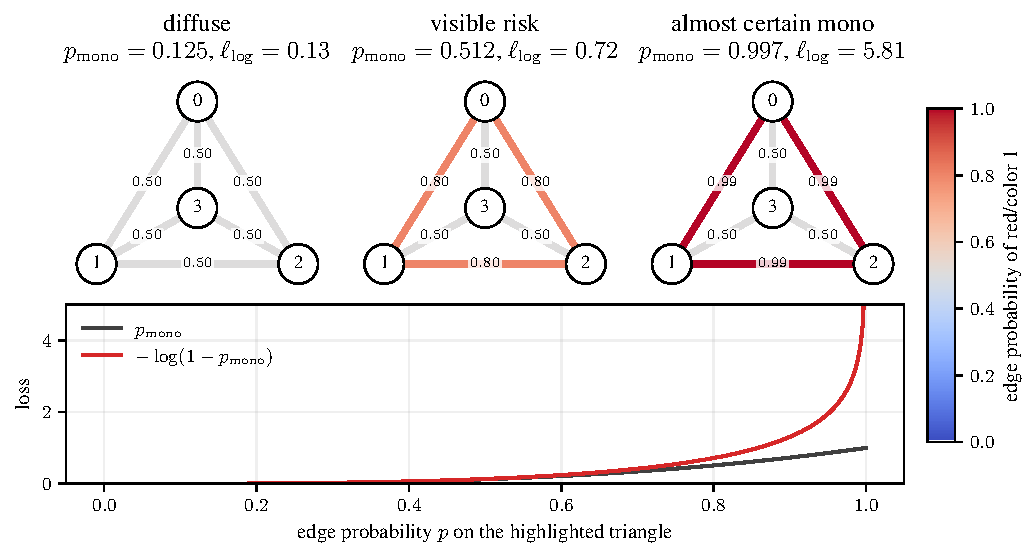
\includegraphics[width=0.8\textwidth]{figures/log_loss_k4.pdf}
    \caption{Effect of the log-barrier surrogate on a toy $K_4$ coloring. As the highlighted triangle becomes nearly monochromatic, the raw product term $p_{\mathrm{mono}}$ remains bounded and changes smoothly, while $-\log(1-p_{\mathrm{mono}})$ grows sharply, concentrating optimization pressure on the dangerous near-violation.}
    \label{fig:log-loss-k4}
\end{figure}

We treat the choice of surrogate as a design decision rather than a theorem-level necessity. The vanilla probability loss $M$ is a natural baseline; in our experiments the log-barrier surrogate empirically outperforms it, with a systematic ablation separating the surrogate from the optimizer and batching strategy left for future work.

\subsection{Frank-Wolfe Updates}\label{sec:fw-updates}

Let $F$ denote the search loss supplied to the optimizer, such as the raw violation count $M$, the log-barrier surrogate $L$, or a piecewise clipped variant of $L$. For smooth losses we use the exact gradient; for straight-through variants we use the specified gradient estimator. We optimize over the hypercube $[0,1]^m$ with a Frank-Wolfe method \cite{frank1956algorithm,braun2022conditional}. At iteration $t$, given a current iterate $x_t$ and gradient or gradient estimator $g_t$, the linear minimization subproblem is
\begin{equation}
    s_t \in \arg\min_{s \in [0,1]^m} \langle g_t, s \rangle.
\end{equation}
Because the feasible region is a hypercube, this oracle has a simple closed form:
\begin{equation}
    (s_t)_{ij} =
    \begin{cases}
        0, & \text{if } (g_t)_{ij} > 0, \\
        1, & \text{otherwise.}
    \end{cases}
\end{equation}

The iterate is then updated by
\begin{equation}
    x_{t+1} = (1-\gamma_t)x_t + \gamma_t s_t,
\end{equation}
where $\gamma_t \in [0,1]$ is a step size.

This update is projection-free and inexpensive once the gradient has been estimated. The oracle returns a vertex of the hypercube at each step, so when initialized at a hypercube vertex (or a convex combination of vertices) every iterate is a convex combination of explicit binary colorings rather than the result of a projection back to the feasible set.

For the exact-gradient version on the smooth raw objective $M$, this update also falls under standard nonconvex Frank-Wolfe theory: under the usual smoothness and step-size assumptions, the minimum Frank-Wolfe gap among the first $T$ iterates decays as $O(T^{-1/2})$ \cite{lacostejulien2016convergence,braun2022conditional}. This is a stationarity guarantee, not a guarantee of finding a Ramsey witness; lower-bound certificates come from conditional-expectations rounding applied to $M$, followed by exact clique verification --- regardless of whether the search step used $M$, a surrogate loss, or a stochastic clique batch.

All experiments reported below use this vanilla Frank-Wolfe update with a standard diminishing step-size schedule. Pairwise and away-step variants are natural active-set baselines, but a careful comparison at this scale is left to future work.

% Move to conclusion / extensions if we discuss multicolor Ramsey variants.
% \paragraph{Remark (multicolor parameterization).}
% Although the presentation above is two-color, the implementation actually operates on a multicolor parameterization in which each edge carries a probability vector $x_{ij} \in \Delta^{c-1}$ over colors. The linear minimization oracle is unchanged in spirit: writing $g_{ij} \in \mathbb{R}^c$ for the gradient on edge $\{i,j\}$, $\arg\min_{z \in \Delta^{c-1}} \langle g_{ij}, z \rangle$ places all mass on a minimizing color, i.e.\ returns a standard basis vector. The oracle still returns an extreme point, now interpreted as choosing one color per edge. This keeps the code compatible with multicolor Ramsey variants, but plays no role in the experiments reported here, all of which are two-color.

\subsection{Stochastic Clique Batching}\label{sec:batching}

The main computational bottleneck is enumerating the forbidden vertex sets. Even for moderate $n$, the number of $k$-vertex subsets,
\[
|\mathcal{C}_k| = \binom{n}{k},
\]
is far too large for exact evaluation at every Frank-Wolfe step. Since the search loss is a sum of independent clique-wise penalties, the natural approximation is to replace this sum by a mini-batch estimate.

Let $\ell_r(C;x)$ and $\ell_s(D;x)$ denote the two per-clique contributions. For the barrier surrogate in \cref{eq:log_barrier},
\[
\ell_r(C;x) = -\log\left(1 - p_r(C;x)\right),
\qquad
\ell_s(D;x) = -\log\left(1 - p_s(D;x)\right).
\]
Mini-batches are used for the search loss, not for the certifying objective $M$. In particular, the implementation uses per-family averages such as
\[
\bar{L}(x)
:=
\frac{1}{|\mathcal{C}_r|}\sum_{C \in \mathcal{C}_r} \ell_r(C;x)
+
\frac{1}{|\mathcal{C}_s|}\sum_{D \in \mathcal{C}_s} \ell_s(D;x),
\]
which balances the average penalty in each color class. In diagonal instances this differs from the raw sum $L$ only by a common scalar factor. In off-diagonal instances it is a deliberate weighting choice: estimating the raw sum instead would require multiplying the two mini-batch averages by $|\mathcal{C}_r|$ and $|\mathcal{C}_s|$, respectively. Rounding and final verification remain defined in terms of the unnormalized violation count $M$.

In diagonal instances, both terms are indexed by the same family of vertex sets, so each stochastic step samples a batch $S\subseteq \mathcal{C}_r$ and evaluates both colors on the same local patterns. In off-diagonal instances, the two terms live on different set families; our implementation synchronizes independent batches across epochs so that both color classes complete one full pass through their respective families at the same time. The detailed batching construction is given in the appendix.

\subsection{Extraction and Verification}\label{sec:extraction}

Lower bounds are certified only after converting a fractional candidate to a binary candidate and verifying directly that no forbidden monochromatic cliques remain. In our implementation this conversion is deterministic and is performed by the method of conditional expectation applied to the raw violation count $M$, regardless of which search loss $F$ produced the candidate. The guarantee is therefore a guarantee for $M$, not for the surrogate loss optimized by Frank-Wolfe.

Starting from a fractional candidate $x \in [0,1]^m$, we process edges one at a time in an arbitrary order. For the current undecided edge $e$, we evaluate $M$ conditioned on fixing $x_e=0$ and on fixing $x_e=1$, keeping the remaining undecided edges at their current fractional values, and permanently fix $x_e$ to the endpoint with the smaller conditional expectation of $M$. Because $M$ is multilinear, and therefore affine in each coordinate, we have
\[
    M(x) \;=\; x_e\, M(x \mid x_e = 1) \;+\; (1-x_e)\, M(x \mid x_e = 0),
\]
so at least one of the two endpoints has value no larger than the current conditional expectation. Iterating this argument over all edges produces a binary candidate $\widehat{x} \in \{0,1\}^m$ with
\[
    M(\widehat{x}) \;\leq\; M(x).
\]
Since $M(\widehat{x})$ is a nonnegative integer, the rounded $\widehat{x}$ is a Ramsey witness whenever $M(\widehat{x}) = 0$; rounding can succeed from fractional points with $M(x) < 1$ (the classical probabilistic-method existence threshold) and also from points with larger expected violation count, and the final certificate is determined by exact clique verification of $\widehat{x}$ rather than by the fractional value $M(x)$. We verify $\widehat{x}$ against the original Ramsey constraints by the clique-checking procedure described in \cref{sec:problem}.

\section{Results}

We evaluate the method on diagonal and near-diagonal Ramsey instances; the global picture is summarized in \cref{tab:small-ramsey-grid}. The pipeline matches the best known lower bound across a broad swath of the small-Ramsey table: it certifies $R(3,k) \geq L(3,k)$ for all $k \leq 8$ (where $L(r,s)$ denotes the current best known lower bound), recovers lower-bound witnesses matching the known exact values $R(4,4) = 18$ and $R(4,5) = 25$, and most importantly reproduces $R(5,5) \geq 43$ by repeatedly finding $42$-vertex colorings with no monochromatic $K_5$ in either color. The $R(5,5)$ recovery is the most demanding entry in the table: it matches Exoo's long-standing $42$-vertex construction~\cite{exoo1989lower} and is a bound that the recent AlphaEvolve-based search does not report~\cite{nagda2026reinforcedgenerationcombinatorialstructures}. The current pipeline does not yet solve every nearby frontier instance; we discuss these limitations below.

\paragraph{Many witnesses.}
A striking feature of the $R(5,5)$ runs is that the method does not converge to a single isolated solution. Across independent restarts it produces a large collection of distinct $42$-vertex certificates, indicating that the optimization landscape contains a nontrivial family of high-quality constructions rather than a single basin. \cref{fig:r55-results} visualizes this as a histogram of how often each distinct certificate class was encountered, identifying classes up to isomorphism and complement; representative graph6 strings are listed in \cref{tab:results}. The shape of the histogram is informative: a small number of colorings are recovered in abundance, while a long tail of colorings is found only one or a few times. So far the method has discovered $81$ of the $328$ known complement classes of $42$-vertex colorings. We do not expect to recover all of them with the current uniform initialization; designing initialization priors that bias the search toward under-represented basins is a natural direction for future work.

To check whether this multimodal pattern is specific to $R(5,5)$ on $42$ vertices, we ran the same experiment for $R(4,4;15)$, an instance for which $640$ inequivalent certificates are known~\cite{mckayramseydata}. The histogram in \cref{fig:r4415-results} has the same qualitative shape: a few colorings dominate the runs while most appear rarely. Together, the two histograms suggest that the multimodality is a property of how the relaxed objective interacts with conditional-expectation rounding, rather than an artifact of one particular instance.

\begin{figure}[h]
    \centering
    \begin{subfigure}[t]{0.48\textwidth}
        \centering
        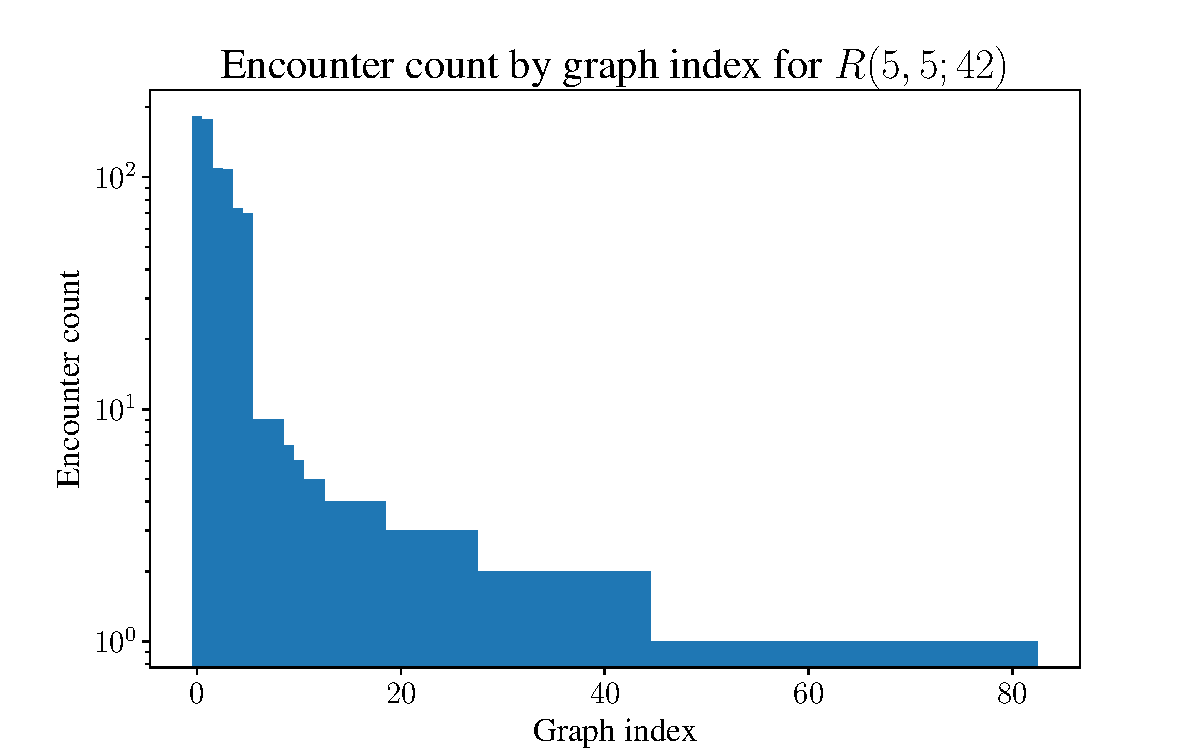
\includegraphics[width=\linewidth]{figures/r5_5_n42_cost0.pdf}
        \caption{Recovered $R(5, 5; 42)$ witnesses.}
        \label{fig:r55-results}
    \end{subfigure}
    \hfill
    \begin{subfigure}[t]{0.48\textwidth}
        \centering
        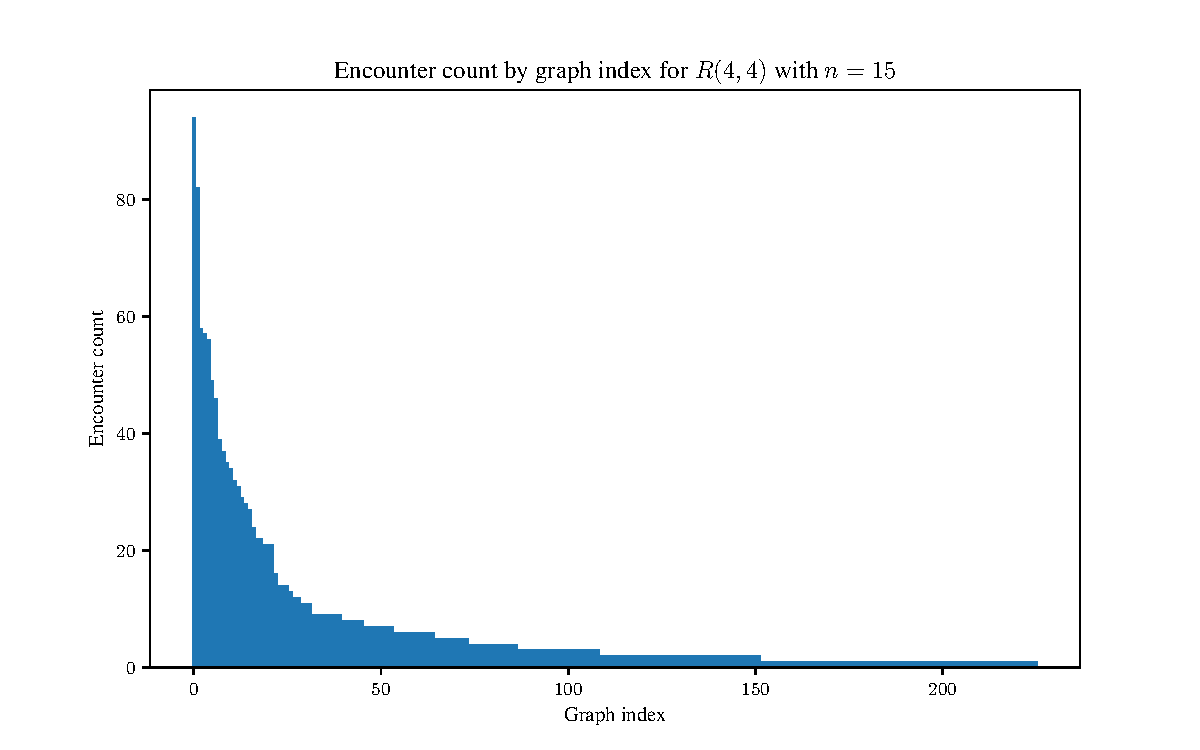
\includegraphics[width=\linewidth]{figures/r4_4_n15_cost0.pdf}
        \caption{Recovered $R(4, 4; 15)$ witnesses.}
        \label{fig:r4415-results}
    \end{subfigure}
    \caption{Histograms of encountered witnesses. Each bar is a distinct certificate class up to isomorphism and complement; the height is the number of independent runs that recovered it. For $R(5,5)$, representative graphs are listed as graph6 strings in \cref{tab:results}. In both instances, a small number of certificates are recovered in abundance while most appear in the long tail.}
    \label{fig:witness-histograms}
\end{figure}

\paragraph{Where the method does not yet work.}
The cases the method does not yet solve are equally informative. In particular, we do not yet report a $35$-vertex witness for $R(4,6)$. Larger near-diagonal cases such as $R(4,7)$ and $R(5,6)$ involve substantially larger clique families and are left for future experiments. These limitations are consistent with the broader picture that the method is currently strongest on diagonal and near-diagonal cases.

\paragraph{Comparison with prior work.}
These results support the paper's central claim: Frank-Wolfe style continuous optimization is competitive with the ad-hoc vertex-by-vertex extension pipelines previously used for these problems, while running directly on the target instance, with current evidence strongest on diagonal and near-diagonal cases. The comparison to LLM-driven Ramsey search should be framed carefully. Recent AlphaEvolve-based work improves or matches many classical lower bounds and is especially strong on larger off-diagonal instances~\cite{nagda2026reinforcedgenerationcombinatorialstructures}. Our method is not an apples-to-apples replacement for that meta-search pipeline; rather, it runs vanilla Frank-Wolfe directly on the violation objective, without program synthesis or algebraic/circulant restrictions on the edge variables, and already recovers nontrivial witnesses --- including $R(5,5) \geq 43$, which AlphaEvolve does not report.

\begin{table}[t]
  \centering
  \normalsize
  \setlength{\tabcolsep}{8pt}
  \renewcommand{\arraystretch}{1.3}
  \definecolor{cellblue}{RGB}{198,226,239}
  \definecolor{cellyellow}{RGB}{255,242,102}
  \definecolor{cellorange}{RGB}{255,165,0}
  \definecolor{cellgray}{RGB}{235,235,235}
  \caption{Results obtained through our method. Blue cells: exact Ramsey number known and matched by our witness. Yellow cells: exact value unknown, our witness matches the current best lower bound. Red cells: our witness falls short of the best lower bound known in the literature. Reference values from the current small-Ramsey survey and graph database~\cite{radziszowski2026smallramsey,mckayramseydata}.}
  \label{tab:small-ramsey-grid}
  \begin{tabular}{c|cccccc}
    $r \backslash s$ & 3 & 4 & 5 & 6 & 7 & 8 \\
    \hline
    3 & \cellcolor{cellblue}6 & \cellcolor{cellblue}9 & \cellcolor{cellblue}14 & \cellcolor{cellblue}18 & \cellcolor{cellblue}23 & \cellcolor{cellblue}28 \\
    4 &  & \cellcolor{cellblue}18 & \cellcolor{cellblue}25 & \cellcolor{cellorange}34 & \cellcolor{cellgray}-- & \cellcolor{cellgray}-- \\
    5 &  &  & \cellcolor{cellyellow}43 & \cellcolor{cellgray}-- & \cellcolor{cellgray}-- & \cellcolor{cellgray}-- \\
  \end{tabular}
\end{table}

\section{Conclusion and Outlook}

We presented a continuous-optimization route to Ramsey lower-bound construction. The key step is to move the forbidden-clique constraints into a pseudo-Boolean violation objective, relax the edge variables to the hypercube, and then use Frank-Wolfe updates whose linear oracle returns binary colorings. The resulting objective is nonconvex and non-monotone supermodular, so the continuous optimizer is used as a search heuristic rather than as a source of global guarantees. Independently, the raw multilinear objective supports exact extraction: it has no integrality gap at the level of global optima, and conditional-expectation rounding converts any fractional candidate into a binary graph without increasing the raw violation count. Final claims are certified by exact verification, not by the continuous optimizer alone.

To the empirical question posed in the introduction --- whether a first-order method on the hypercube relaxation finds useful discrete witnesses in practice --- our experiments give a partial yes. This simple pipeline recovers a substantial part of the small-Ramsey lower-bound table and repeatedly finds $42$-vertex witnesses for $R(5,5) \geq 43$, without imposing circulant, algebraic, or other structural restrictions on the graph. The multiplicity of recovered witnesses, especially for $R(5,5)$ and $R(4,4;15)$, shows that the search dynamics reach multiple basins leading to valid certificates rather than a single isolated construction. At the same time, the method is not yet a universal Ramsey-search engine: nearby cases such as $R(4,6)$ remain unsolved by the current implementation, and larger off-diagonal instances introduce much larger clique families.

Several directions follow naturally. On the algorithmic side, active-set variants of Frank-Wolfe, alternative step-size rules, and initialization priors could change which witness basins are reached. On the modeling side, sharper ablations of the raw objective, log-barrier surrogate, clipping convention, and batching scheme would clarify which ingredients are essential. The same template also has concrete Ramsey-theoretic extensions: multicolor problems replace each edge variable by a simplex vector whose LMO still chooses one color per edge; ordered and canonical variants change the indexed forbidden-pattern family; and Ramsey multiplicity changes the target from zero violations to minimizing a certified monochromatic-clique count.

\newpage

\bibliographystyle{abbrv}
\bibliography{bibliography}

\newpage


%%%%%%%%%%%%%%%%%%%%%%%%%%%%%%%%%%%%%%%%%%%%%%%%%%%%%%%%%%%%

\appendix

\section{Technical appendices and supplementary material}
The appendix collects implementation details, additional ablations, proofs for any formal statements about the batching scheme, and supplementary visualizations of recovered colorings. It also includes extended witness statistics and additional instance-by-instance results that are useful for reproducibility but not essential to the main narrative.

\subsection{Detailed batching scheme}

For batching, it is convenient to work with the vertex-family-averaged search loss
\[
\bar{L}(x)
:=
\frac{1}{|\mathcal{C}_r|}
\sum_{C \in \mathcal{C}_r} \ell_r(C;x)
+
\frac{1}{|\mathcal{C}_s|}
\sum_{C \in \mathcal{C}_s} \ell_s(C;x),
\]
where $\ell_r$ and $\ell_s$ are the per-clique terms of the chosen search loss. This normalization is part of the optimization objective being sampled. When $r=s$, it differs from the raw sum by a common scalar factor. When $r\neq s$, it changes the relative weighting of the two color classes compared with the raw sum; this balances average per-family penalties during search, while extraction and certification still use the raw violation count $M$.

The diagonal case $r=s$ is straightforward. Both color terms are indexed by the same family of $r$-vertex sets, so we sample a single batch $S \subseteq \mathcal{C}_r$ and evaluate both colors on that same set:
\[
\widehat{L}_{\mathrm{diag}}(x)
:=
\frac{1}{|S|}
\sum_{C \in S} \bigl(\ell_r(C;x) + \ell_s(C;x)\bigr).
\]
This is an unbiased estimator of $\bar{L}(x)$. Using the same batch for both colors is also the most intuitive choice: each stochastic update compares the red and blue penalties on exactly the same local vertex pattern, rather than adding variance from two unrelated samples.

The off-diagonal case $r \neq s$ requires one more design choice because the two color terms live on different vertex-set families. Here the main question is not whether to batch, but how to organize the two batches across an epoch.

Let
\[
R = \max(r,s), \qquad q = \min(r,s),
\]
and let $\ell_R$ and $\ell_q$ denote the per-set penalties for the corresponding two colors. We choose a batch size $B_R$ for the larger vertex-set family $\mathcal{C}_R$, and define
\[
T = \left\lceil \frac{|\mathcal{C}_R|}{B_R} \right\rceil
\]
to be the number of optimization steps in one epoch. At the start of the epoch, we randomly permute all $R$-vertex sets and partition them into batches
\[
A_1,\dots,A_T,
\qquad |A_t| \leq B_R.
\]
We then independently permute the smaller vertex-set family $\mathcal{C}_q$ and partition it into the same number $T$ of batches
\[
B_1,\dots,B_T,
\qquad |B_t| \approx \frac{|\mathcal{C}_q|}{T}.
\]
Equivalently, the smaller-family batch size is chosen so that both colors finish one full pass through their respective vertex-set families at the same time.

At optimization step $t$, we evaluate one batch from each color and then apply a single update:
\[
\widehat{\mathcal{L}}_t(x)
:=
\frac{1}{|A_t|}
\sum_{C \in A_t} \ell_R(C;x)
\;+\;
\frac{1}{|B_t|}
\sum_{D \in B_t} \ell_q(D;x).
\]
This is what ``independent batching'' means in our epoch-based implementation. The two color classes are sampled independently, but they are synchronized at the level of epochs: each step uses the $t$-th batch from the large-clique pass and the $t$-th batch from the small-clique pass, and after $T$ steps both passes are complete.

This viewpoint is often clearer than thinking of each update as drawing two fresh random mini-batches from scratch. Over one epoch, every set in each family is visited exactly once, up to the usual rounding in the last batch, and reshuffling happens only when the next epoch begins. The resulting estimator is still unbiased for the same vertex-family-averaged objective, while fitting naturally with the ``one pass through all vertex sets per epoch'' interpretation used in the implementation.


\section{Detailed results}

\begingroup
\setlength{\LTleft}{0pt}
\setlength{\LTright}{0pt}
\setlength{\tabcolsep}{3pt}
\scriptsize
\begin{longtable}{r >{\fontsize{4}{5}\selectfont}l r}
    \caption{Detailed results for $R(5,5)$.}\label{tab:results}\\
    \toprule
    idx & graph6 string & occ. \\
    \midrule
    \endfirsthead
    \multicolumn{3}{l}{\tablename~\thetable{} (continued)}\\
    \toprule
    idx & graph6 string & occurrences \\
    \midrule
    \endhead
    \midrule
    \multicolumn{3}{r}{Continued on next page}\\
    \midrule
    \endfoot
    \bottomrule
    \endlastfoot
        0 & \texttt{ipUR`?\{mFxYm\textasciitilde{}F@vNE\_KvuwfX`O]t[\textasciicircum{}FMNbw\textasciitilde{}QWE\textasciicircum{}w?ZwH\textbackslash{}[WDZxkJMCQavzqA\textbackslash{}ukxbQTaD\textbackslash{}W\textasciitilde{}sDjKKlb\}BbctrOMGvesin\}iGlA@heVmNNvObTOSzaEgmKN]BPoOB\textasciitilde{}VC[BaE|\textbackslash{}[AfCg\}aLp\_} & 162 \\
        1 & \texttt{icGA|Mi@zyBvceVW[RyrEsQR\{\textasciicircum{}\}?FabFrQeh\textbackslash{}MGjz\{TuRzQ\textbackslash{}zaojme\{\textasciitilde{}aaWd]GvonHX|A\textbackslash{}cu\_pVbJdlJuwJLuPFueZr\}@IEZdQHWx\textasciicircum{}QTQJ]sElsSdXUerhTgg]\textasciicircum{}DBs`wpB[bMrQSElaMbM\}@\_} & 156 \\
        2 & \texttt{i]]f`D\textasciicircum{}tKXVMPraG\}ZL@aKUstZDQlFV\_|TPVTQuo\textasciitilde{}p\{Gpbs\textbackslash{}WtM\textbackslash{}DbtHplE\textasciitilde{}yJoVlQEnbzCC\{LxqY\_K[Ngg\textbackslash{}INVombNmHsSDZeX\textbackslash{}SN\textasciicircum{}cKOCtIllLJg\textbackslash{}QF[Z@sZ`WIcS\textasciitilde{}YERz\textasciitilde{}o?wB`JrafPS\_} & 96 \\
        3 & \texttt{iMNdeRs\textbackslash{}u|u\{TLz`fk?\textasciicircum{}CBwgt?ParXQznG\{qSb\textasciitilde{}CQyXEHJv\{k\textasciicircum{}cqwlixAr\{eTDZXjeze?\}g\textbackslash{}eTM\{balw\{I\textbackslash{}BFo]Ixf\_le]RMDZic\{\textasciicircum{}GJe`uRooyL]\textbackslash{}WN@qbdm\}@P`wFo\textasciicircum{}JCoxMTXHXBVIjZOO} & 94 \\
        4 & \texttt{is\textasciitilde{}\{a\textbackslash{}ycYXiY[ohZgLLCjkGWFfruxqD[UvMxH|\{?tiQwxDlpR\}W`Vh?f\textasciitilde{}F\}BscOy\}kMtCY\textasciitilde{}LR@y\textasciicircum{}vONoH\{]AUHlTs\}E\_HlIRkJHHqqYR?WxU\_cQpYXMETpl\_YdyHsXoMYqw\_apQuNd\_sSJW\textasciicircum{}g} & 62 \\
        5 & \texttt{i[\{?PeLGo\textasciicircum{}\textasciicircum{}\textasciitilde{}kg@sJSNtRr]zYjBwvIysjupG|E\{VibN\{iEoBLv\_|XYBUegMbALJhwnkGBNF\_ByywVLs\_LvKtRfkgx\}uaWp@kOR\textasciicircum{}Y\_\textasciicircum{}?vydWmzsAsd]\textbackslash{}p[GFhaRpJuSExvgI`ikf\textbackslash{}H\_mRTUJX?} & 59 \\
        6 & \texttt{iE`\textasciitilde{}r]HrhceF@b?C\textasciitilde{}\textbackslash{}XpmvR\textbackslash{}wnVQMfUShTob|\textasciitilde{}o@`qU[U\textbackslash{}C`ppZhqTjBs\textasciicircum{}FDwupiuTRfA[cNuBbrgxNGMNi[eTpz\_UJ\_iyJrAuSMzxQo]EyXPRqdsmDy\textbackslash{}ICnt@vhSMNSe\textbackslash{}SQnJYELAkIrepPG} & 9 \\
        7 & \texttt{iipz|M\{iREvHbNS\textasciitilde{}cLM\_rUIyBvty`uSFXHqQgNapLVEzZfBc|\{WbMQKmWoTPjdqFlbT@XB]dg\{\textasciitilde{}@\textasciitilde{}\{DwGREz\{\_yq`Ft\}f[Bwp\{BwN`oL\_WH\textbackslash{}`\textbackslash{}A`q`Sg\}E[WDj`LqL?LqJ\textasciicircum{}oBPUXXsowS`|fG} & 9 \\
        8 & \texttt{ilCe]JYQqSE\textasciitilde{}jY|E\textasciicircum{}clxwCsiewHvOHvsRK`ZRTvcHNNM\}wkEQ\textasciicircum{}syDEJbJSvIEvsB\textasciitilde{}?mqTs`YrvmqgUF]?\textasciicircum{}oyv]BIbRjYKqO\_zrXl|Lqqbak[bhwaLgj[LDp\textasciitilde{}\}?BwMC]I|?[sRKFwKcgPnnI\_W} & 7 \\
        9 & \texttt{iGgRNqIvLu\_@U`F`BhLnGFagT\textasciitilde{}HJi\textasciitilde{}Wnr\textasciitilde{}ctK\textbackslash{}|FbFK]CxAx\textasciitilde{}\textasciitilde{}?@VmjY\textasciitilde{}?\textasciicircum{}esLSqeb\{GnkLXErx|aeDVFG\{fuDYW\{v`orIVQdKjdLvBXbIlNEFVDqgZdPMH\textasciitilde{}wkHHMFBZSkQGVB|ZL@oqqlBBo} & 6 \\
        10 & \texttt{irDva\_P\}kNPsiXiRLDVXGFucT||ibMcNdS\textasciicircum{}RUBzt\textasciicircum{}?mc]EVPcwZb\textasciitilde{}\{?P\{tcRRYULFn?\textasciicircum{}R|OsVE\textasciitilde{}?sVThsrJBhBC\textasciicircum{}uxQhw\textbackslash{}bb\textasciicircum{}PkR]pz?r@]XmqEPaeVij[JEKR]QXK\textasciitilde{}LELHQtFVDRAahhsxQG} & 5 \\
        11 & \texttt{ildmjMjnSvJfyw\textbackslash{}FGTxPnYqOdl[h\{d`VJWFQrbNqZLPYqNlUmaGkslYibIqTUDOtb\{N\textasciitilde{}oxwowrWsGVGmxjYMZd`ATTWbo\{LIIDXdTRhWeXK]AtaFo@rsKl\{aVyaBReB`RLpr`?Gp\textasciitilde{}SobIiujG} & 5 \\
        12 & \texttt{irmknDZV]nS\{ZD]D|ILS\{mYBcJ|cZOdnTBNiPmjG\{VzLx`\_TXWTb\{N\textasciitilde{}qE]aCyNcDhwohITi?uxRl\textasciicircum{}orSiaX`[[HSrWmEpbUIkfUIFSeO\}BuEKyhFpSb@MkW@YWRnh|GHo\textasciicircum{}A[WRMI[sqHSUldo} & 5 \\
        13 & \texttt{iLEjSSO\textbackslash{}\textasciicircum{}VxAft|?W\textasciicircum{}EjNDj\textasciicircum{}\_Lil]WY\textbackslash{}gWlD\textbackslash{}pm\_WxuOpeFmnPjG\textasciitilde{}RUFvXeCmUMHX|\{aBjdbCse\_F|bjfQyFk\_\textbackslash{}`yjcoj`IH\_\textbackslash{}C|fYBXhVVG\textbackslash{}XTvY\textbackslash{}jNLeZK[ch[eS[HyQL\}IKOlMIbtZbKBw} & 4 \\
        14 & \texttt{iOH@jJZaofDdqtg@jLfw\textasciitilde{}hMYiSBlfMumXtzCf\{XKyYT\textasciicircum{}`TgvqXav`JNmqM\textasciicircum{}ElLyA]o\}`Br[[?\{xyaxQNouwSvMTdH\textasciicircum{}TYRL@P\}Pmh[\textbackslash{}WQYdi[JiitMox]atXtwvACUXSw[LH`L]cyUPpWFfsGo} & 4 \\
        15 & \texttt{iDFCbtVFcOL]zrLMTCmgoot\textbackslash{}sGTTJ\{VpmwAaSgjn]c`tf`EdldOfethFMlLVuilo\textbackslash{}Jplrg\}[IBBVIKxGVgwo\_xRdfzjmLCrmSJeJIkMIylp\{INhYaBRxjGDLfD\_xqwaQK\textbackslash{}jssN]G`][HeJrPo} & 4 \\
        16 & \texttt{icDlRooF`aMHnA\textasciitilde{}cXVv\{F?xx\{Q\_E]\textasciitilde{}Zgfk\{Ih|FKNo\}Zth\_p\textasciitilde{}w?zyAUjF?V]esJ[\textasciicircum{}HAZkeheN[rhbcq`m\{LK\_\textasciitilde{}|WbvPDmW\textbackslash{}Us\textasciicircum{}\_w]Qtq\_qKY\{tHdvyiHXAF\{|?ZHARraL@m`AvnUGZaTFgbMO} & 4 \\
        17 & \texttt{i?o\{BvyW\{Kw|MBD@\textasciicircum{}VHs]rs|yJVkefl\_hH[b\}\textasciicircum{}oF`ZPQmWlh[TiFy]KVWjFU[m[oaqb\textasciitilde{}?\{elQfaENspJNbm@]IAfTZeUpAmv\_kNJ[rWhqDrJDwzSLViB\textasciicircum{}dLbmbHQcbfSkqhPjjWLYAr?rleaG} & 4 \\
        18 & \texttt{icDlRooF`aCt[QnA\textasciicircum{}qeT\}\textasciitilde{}\_[Bbp@\textasciitilde{}zwicBNlz[anXsHS\}Px`\textasciitilde{}B\{vjhOW\textasciitilde{}\}?F\textasciicircum{}WGlUM?jnR\textbackslash{}@ZbxKGv[rcsxLOvn`hvOazeLUyJwK]QykgIKZ]LQTvzTAUAF\{]\_EtARpsbOm`AZzt\_ZaQ`yHmO} & 3 \\
        19 & \texttt{iMne\textasciitilde{}Y|TWW`a\textasciicircum{}c|nE`@gI\}R\textasciitilde{}GX\}@\textbackslash{}heL\{rKSoNgYvxoXAmEoit\textbackslash{}KrGvrbEnd]lbPrBytEmyEMBWhk\textasciicircum{}H\{ZPMHpbQjFGyk|@sFLLNpY]@\}FELVFKQRlkiKYIa|MLQqFUECyEhQ\textbackslash{}bplArGlUXHoo} & 3 \\
        20 & \texttt{iOf?AZA\}vfVc\}d\textasciicircum{}e\textbackslash{}U@x`gOvF\textasciitilde{}r\textasciitilde{}?O\textbackslash{}qO[iw[Ty\}fYd?xuX\{pMSYteXVZ?zTn?\textasciicircum{}@jUViBZC\{NnGThyAJfq\textbackslash{}p|h@tqnJKdSNgIFwsL\textbackslash{}LOwReJYwqbU\_rqv@EfzcEiILKjeH\{ddiJmoOJubUBy?} & 3 \\
        21 & \texttt{iDFCbtVFcQL]zrLMTCmgoot\textbackslash{}sGtTJ\{VpmwAaSgjn]c`td`EdldOffthFMlLVuilo\textbackslash{}Jplrg\}[IBBVIKxGVgwo\_xRdfzjmLCrmSJeJIkMIylp\{INhYaBRxjGDLfD\_xqwaQK\textbackslash{}jssN]G@][HeJrPw} & 3 \\
        22 & \texttt{iCUVWCkJQ[ETjT?X\{pfb\textasciitilde{}C\}Whs@D\}UtfGfonzTrEluLNyKp\textbackslash{}RQY\{Yjc\textasciicircum{}hK\{VqH[\textasciicircum{}uK[\textasciicircum{}bZE\}OVXFrAEZw\{?\textbackslash{}r\textbackslash{}OvIfeE\textbackslash{}oix[kqc\}elEXgbyoxLQZGxFglvXwlo`DeSwFBTCt]pMdRCwFX|?o} & 3 \\
        23 & \texttt{ildmjMjnSvJfyw\textbackslash{}FGTxPnYqOdl[h\{d`VGpwJu@saZLOyqNnUmaKkslUibIoTUDOTb\{N\textasciitilde{}pkYCJe[G@eGmxiyMZd`ARTWbw\{lIIDxlTRh[exrbNwM?o@rwLl\{aV\{aBReB\_rLpKGqmliOxwoWv\_W} & 3 \\
        24 & \texttt{icGDGL\}FY\{[NUasi\textasciicircum{}ny\}goB`QNBjGR\textasciitilde{}aUpzY\textbackslash{}kVDZE\{\textasciitilde{}iPcjcvoiU`uQKvnDwx\textbackslash{}Afdi@ojKuVLNV@ZZiP|gXm\textasciitilde{}OcorpPH]JuEtsDQrXZJgjeBfcS]P\{p?uPlKh[FZ@gzlwKsDTqvQbJaXRat?} & 3 \\
        25 & \texttt{igELvFh\_N|mWPGF?aYTij\textbackslash{}fRF[hxwqr]PhAtU?I[Ij\{LEKI`Tfk|ussV\}MQc[LQoczw\textasciitilde{}Di[feJcF|\{`\textasciitilde{}eLw|@zsFIFIWDpLRkFE`\}qHumKGNU\textasciicircum{}pFpVaLfKPI\{FEf[hFCXSr\{`dE\{aSMaszosW} & 3 \\
        26 & \texttt{iYRVC|z\{oYdbOR?Cv|X[mtj[\}NStMcvShsob\textasciitilde{}\textasciicircum{}o@WqUVI\textbackslash{}CoXpZqYTjKw\textasciicircum{}FE[upidlRfBeCNu@xrgxMoMNi\textbackslash{}HTpz\_Lb\_iyH|AuSMy|Qo]EmhPRqdlUDy\textbackslash{}ILFt@vhUBNSe\textbackslash{}SKvJYELBIIrepPG} & 3 \\
        27 & \texttt{iLEjSSO\textbackslash{}\textasciicircum{}VxAft|?W\textasciicircum{}EJLDj\textasciicircum{}\_Lyl]WY\textbackslash{}gWlD\textbackslash{}pm\_WxuOpeFmnpjG\textasciitilde{}RUFvXeCmUMHX|kaBjdbCse\_F|bjfQyFk\_\textbackslash{}`yjCoj`IH\_\textbackslash{}C|fYBXhVVGTXTvY\textbackslash{}jNLeZK[ch[eS[HyQL\}IKOlMIbtZbKBw} & 2 \\
        28 & \texttt{iLEjSSO\textbackslash{}\textasciicircum{}VxAft|?W\textasciicircum{}EJLDj\textasciicircum{}\_Lyl]WY\textbackslash{}gWlD\textbackslash{}pm\_WxuOpeFmnpjG\textasciitilde{}RUFvXeCmUMHX|\{aBjdbCse\_F|bjfQyFk\_\textbackslash{}\_yjCoj`IH\_\textbackslash{}C|fYBXhVVGTXTvY\textbackslash{}jNLeZk[ch[eS[HyQL\}IKOlMIbtXbKBw} & 2 \\
        29 & \texttt{iLEjSSO\textbackslash{}\textasciicircum{}VxAft|?W\textasciicircum{}EjLDj\textasciicircum{}\_Lyl]WY\textbackslash{}gWlD\textbackslash{}pm\_WxuOpeFmnpjG\textasciitilde{}RUFvXeCmUMHX|kaBjdbCse\_F|bjfQyFk\_\textbackslash{}\_yjCoj`IH\_\textbackslash{}C\textasciitilde{}fYBXhVVGTXTvY\textbackslash{}jNLeZK[ch[eS[HyQL\}IKOlMIbtZbKBw} & 2 \\
        30 & \texttt{iRrC\}zl@ZMfaNCZeWvrGG\textbackslash{}?jHN\{tb|oxxbB\textasciicircum{}cNsGV\{\{RBVAcjY\textbackslash{}Wpcnrab\textasciicircum{}e\}epPjB|LFmt@MBWsq\textasciicircum{}I\{LkMHphiJF[xUL@tfEaNpU\textasciicircum{}?\}FETTbsQRtkTcYIa\{fTQqFUR?yEhI]pXlAqgmhXHoo} & 2 \\
        31 & \texttt{iLEjSSO\textbackslash{}\textasciicircum{}VxAft|?W\textasciicircum{}EjLDj\textasciicircum{}\_Lyl]WY\textbackslash{}gWlD\textbackslash{}pm\_WxuOpeFmnpjG\textasciitilde{}RUFvXeCmUMHX|\{aBjdbCse\_F|bjfQyFk\_\textbackslash{}\_yjCoj`IH\_\textbackslash{}C|fYBXhVVGTXTvY\textbackslash{}jNLeZk[ch[eS[HyQL\}IKOlMIbtZbKBw} & 2 \\
        32 & \texttt{ipUjSdhWcdqKZv|`|jd\textbackslash{}CEYwhlAjozq?ohj\textbackslash{}dnBPLbmQ\}a[yc[tTVD]zqfdCc\textasciicircum{}Nkpzckrs\{B\{Fp\textasciitilde{}w?]xmBRXNoL\textbackslash{}SrSyfCJxA\{e\_pxxbSD@tkL\textbackslash{}s]FDpYafWshUVDerpHYI[GYyk\textbackslash{}AFGnNGKg} & 2 \\
        33 & \texttt{iDShNSPxNT[WCMzXmy\textasciicircum{}\textbackslash{}keI]iielW\textbackslash{}PRYT]KD\textasciicircum{}\_rQhdysolrl]kVtfO\textasciicircum{}OoqmJuFX|f\_\{?nXB\textbackslash{}vo\textasciitilde{}w@y\{\textasciitilde{}AIpNkKuG]gA\textasciicircum{}IZwP\textbackslash{}\textbackslash{}GP\}\textbackslash{}dGDcO|\}\_M@Xs\textbackslash{}zof[Y`WVTbhqbyG[aMqo\textbackslash{}aFo][O[g} & 2 \\
        34 & \texttt{ilVBaxSudJx\textasciitilde{}hyjyE\}Z[]qJWy[OU\textasciitilde{}tZiqTs\}MRz@b\textasciicircum{}ILgQzVoL\_\}cADxuPHqdTWidYDnysBubDSs\textbackslash{}NxmcEdiip@RPwBCYzJFHHsXkWhYeWSL?I\textbackslash{}|rc\textbackslash{}GCMkkHDGl\{\_viOgveMidiXA[aHLPdw} & 2 \\
        35 & \texttt{iDFCbtVFcQL]zrLMTCmgootLsGtTJ\{VpmwAaSgjn]c`td`EdkdOffthFMlLVuilo\textbackslash{}Jplrg\}[IBBVIKxGVgwo\_|RdfzjmLCrmSJeJIkMIylp\{INhYaBRxjGDLfD\_xqwaQK\textbackslash{}jssN]G@][HeJrPw} & 2 \\
        36 & \texttt{iZbYdo?VC\{?RQbXTl\textbackslash{}LnLVq\}\textasciitilde{}RGFJm`NK@ihmLZPG\textasciitilde{}sIQsMsXdwNfCZdlo\}CL`Xhslp\_\textasciitilde{}uJUIbqqQq`VXD|JEwWfYc\textasciitilde{}@xC`ZMtbG`\textasciicircum{}]Fx@|HPQYJa\}?jA|\textbackslash{}C?Iy\}||gasquyqG\}LkbKQgK\textasciitilde{}Eg} & 2 \\
        37 & \texttt{ihjZvbpwNH@r\{pb\}D\{s\textasciitilde{}ocPvG\textbackslash{}\textasciitilde{}tAvi``Hy\textasciicircum{}FqkJ[WbBvz\_ldYV\textbackslash{}Bg\{PW[HZ\{oWgS\textasciicircum{}\_pMD\{e?z\_nWtU\{K[Fzx?mo]AX]`MxppyoswqRFQToasrZCJIPixOcTcQmmSImAyGNC\textbackslash{}Z]oBSbr@hedo} & 2 \\
        38 & \texttt{igELvFh\_N|mWPGF?aYTij\textbackslash{}fRF[hxwqr]PhAtU?I[Ij\{LEGI`Tfk|ussV\}MQc[LQoczw\textasciitilde{}Di[feJcF|\{`\textasciitilde{}eLw|@zsFIFIWDpLRkFE`\}qHumKGNU\textbackslash{}pFtVaLfKPI\{VEf[hFCXSr\{`dE\{aSMaszosW} & 2 \\
        39 & \texttt{iRCHEVUp@FDmufZRzzddFdjRmo[dMtRoojwEtcoYajJ|r@Xvs|W\textasciicircum{}UMc]b`cmVSMxz\textasciicircum{}@w?\textbackslash{}eE|pk\textbackslash{}OuFb\textasciitilde{}o@||zADWVkE\textbackslash{}abkGfXTsYmUNs]HVRh\_fquUODs@\textbackslash{}\textasciitilde{}OROStFnZ@XH\textbackslash{}aoMYN?\{\{QJG} & 2 \\
        40 & \texttt{iRCOTWCsV\_XlklHmdVYalJMVVcmvIO[sZm`r\textasciitilde{}loffYa|\textasciitilde{}o?f\}CU\textasciitilde{}`PL@mTZjESqzdwhx`xIueJnuAM?Tzo[\textasciitilde{}o]laHvHMwo\textasciicircum{}PW\}?YUiJuEpgLuYfEXeLw[b|wN\_MFAvAK[sJFbhVHMb@Xyxa\_o} & 2 \\
        41 & \texttt{iajtD\_\textbackslash{}WOBhzXMRn]f[mRGxTHNmxqxwjUA\_huh\{JdphQlyEEicKs]NwUVad\}\}gI\textasciitilde{}XUpTkyBlw\textbackslash{}\}I\_C\textasciitilde{}]kRWENoAdAy``Dh[eouSbB\{OKP\textasciitilde{}\textbackslash{}O@Nz\textbackslash{}IGzRykPAVLSDjW\{u[D`KwBi\_m\textasciitilde{}gmMwDLo} & 2 \\
        42 & \texttt{iajtD\_\textbackslash{}WOBhzXMRn]f[mRGxTHNmxqxWjUA\_huh\{JdphQlyEEicKs]NwUVad\}\}gI\textasciitilde{}XUpTkyBlw\textbackslash{}\}I\_C\textasciitilde{}]kRWENoAdAy``Dh[eouSbB\{OKP\textasciitilde{}\textbackslash{}O@Nz\textbackslash{}IGzRykPAVLSDjW\{u[D`KwBi\_m|gmMwDLo} & 2 \\
        43 & \texttt{iGhfsZXng?j`FAEcux?wiC\textasciitilde{}cbi\textasciitilde{}P\textasciicircum{}f\}RSrng\{prFa[`[\textasciitilde{}\textasciitilde{}??n\textbackslash{}Ut\{@\}Z`ieOhF\}MfFwPZgYqLrrzDKd]MPxFsIsp\{vB`eUVTIXVDLmErFIk]KMnDrOvI`MWwZYcpHDo\textasciitilde{}UXg[XXU\_oxN\}JAHHG} & 2 \\
        44 & \texttt{iMo|fBVxtuiJBpBpN[fb]MO\_|@Vcf\}[K\{wpnJMjMG\textasciicircum{}PiVxop`VEpIlYfEXD\{mKZ[h|ZHFJByiLV\textbackslash{}AmBUIYncvbYRalZIeLBwpgJFpfLG\textasciicircum{}bvN?\}FALTpqHLanRehWFT`\_|BDQfWwudRIJT[cgo} & 1 \\
        45 & \texttt{iUW]gIfLUIpik`oenDpv[YTuuWm?V`k\}UHl@Vs[kvbF|ghMSUft[iVOlxqRMRkbCvmC@hbkgXXaFkikLj[JbksGY[JkhZ[NJ\_pH]\}IWmB\textbackslash{}?u\textasciicircum{}jR`OH\textbackslash{}p|vTZs\textbackslash{}DlBsN[DiKlAbne\{q\textbackslash{}mvpLO?} & 1 \\
        46 & \texttt{iYPE`\textasciicircum{}\_fjp\}MJ`@PVvH\textbackslash{}Msy\{\}bSzUczohqKb\textasciitilde{}foDwjPWjWlqUTiX\{]KXsjFSf][owgb\textasciitilde{}?NUlQewENsqQnbm?vaAfTMyUpAmlokNJVLWhqDktDwzSZRiB\textasciicircum{}dFXmbHQeGvSkqhK\textbackslash{}jWLYBK\_rleaG} & 1 \\
        47 & \texttt{icDlRooFbaV\_\textasciitilde{}cqn\textasciicircum{}owF]\textasciicircum{}DOBM\textasciitilde{}ZpNXogpfeh\}M[N`\{ZtRCp\textasciitilde{}o?zwCejE?n]egU[KRPZ|\{gRMsrrFch\textasciitilde{}]`Ej\textbackslash{}Glx\_itFsFVcyxgDZ\{iGlAHgrJvFQ[whiJIFv\_s[@@\textasciitilde{}spDB`@nVVPFaYNgaX\_} & 1 \\
        48 & \texttt{iUW]gIfLUIpik`oenDpv[YTuuWm?V`k\}UHl@Vs[kvbF|ghMSEft[iVOlxqRMRkbCvm?@hbkgHXaFkikLj[JbksGY[JkhZ[NJ\_pH]\}IWmB\textbackslash{}Au\textasciicircum{}jR`OH\textbackslash{}p|vTZs\textbackslash{}DlBsN[DiKdAbne\{q\textbackslash{}mvpLO?} & 1 \\
        49 & \texttt{iUW]gIfLUIpik`oenDpv[YTuuWm?V`k\}UHl@Vs[kvbF|ghMSUft[iVOlxqRMRkbCvmC@hbkgHXqFkikLj[JbksGY]JkhZ[NJ\_pH]\}IWmB\textbackslash{}?u\textasciicircum{}jR`OH\textbackslash{}p|vTZs\textbackslash{}DlBsN[DiKdAbne\{q\textbackslash{}mvpLO?} & 1 \\
        50 & \texttt{i[XDvxcNUjNVZKbo\}[HHYXTegb|KIY`fXZ]YGm@qLiux`\{HkbtFFocq?JDYLJwDtVtwQWgDulM@PxdI\textasciitilde{}BGhAAcprrPfE\_\textasciicircum{}\{\textasciitilde{}C\textbackslash{}JnRR@uauc?l\textbackslash{}pZSyUTiTfw\textasciicircum{}[YcD`tBZeQ\{KEfj`S\textasciicircum{}\}?\textbackslash{}`UO} & 1 \\
        51 & \texttt{ir[XowSCQDXfbkk`\}HzBuLZCt\textasciicircum{}BHqMKezBrM|\}GF\textasciicircum{}\}?P\{Fwb\{mgvbVsDPm]VqTbXaKi\textasciitilde{}@pvYhTrhOVVwo[pPriNcoz\_UhqvGwzDVZ\textbackslash{}GFoc`tGVwVHV\textasciitilde{}ECXW\textbackslash{}Mwoai[DFjuOEnxDFgGosVRmQO} & 1 \\
        52 & \texttt{i\{XDuxcNUjNVZKbo\}[HHYXTegb|KIY`f|Z]YGm@qLiux`\{HkbtFFo\_q?JDYLJwDtVtwQWgDulM@PxdY\textasciitilde{}BkhAAcorrPfE\_\textasciicircum{}\{\textasciitilde{}C\textbackslash{}JnRR@uAuc?l\textasciicircum{}pZSyUTjTf\{\textasciicircum{}[YcD`tBZeQ\}KEfj`S\textasciicircum{}\}?\textbackslash{}`UO} & 1 \\
        53 & \texttt{iMqamd]m\}yA\textbackslash{}\}b\textbackslash{}OFg`yIT?Ih|IHezHvUbxaAf\textasciitilde{}AGd|x[\textasciicircum{}qjpYhgjMyTWjLNpms\_]SNZJ[\{`qn`wYYC\textasciitilde{}@sJewDmRqV`U]hLHspTfSrowyKXypMBfKUz\{DCM?\}`xXe\textasciicircum{}cArOibq[UqOsMmQeug\_} & 1 \\
        54 & \texttt{iZbYdo?VC\{?RQbXTl\textbackslash{}HnLVq\}\textasciitilde{}RGFJm`JK@ilmKZPG\textasciitilde{}sIQsMsXdwNfCZdlo\}cL`Xhslx\_vuJUIbqqQq`VXD|JFwWfYc\textasciitilde{}@xC`ZMtbG@\textasciicircum{}]Fx@|HPQYJi\}?jA|\textbackslash{}C?Iy\}||gacquyqG\}LkbKQgK\textasciitilde{}Eg} & 1 \\
        55 & \texttt{iuiCA\textbackslash{}guE|]KL\{\textasciicircum{}lMtHn`nF\}xw\_|jJ\{?aDqj\_\{MsIrhhpojPr\textbackslash{}X?rp\}LoqlndDRtNWE|TpmNDJyKobAyQ]FUUyRdF]s\_NfardjTCPwhrpsyNct?zxn@g\{BFImhqaKD\textasciicircum{}Py]ChkscgMZj\textbackslash{}\_HpWG} & 1 \\
        56 & \texttt{iZbYdo?VC\{?RQbXTl\textbackslash{}HnLVq\}\textasciitilde{}RGFJm`JK@ilmKZPG\textasciitilde{}sIQsMsXdwNfCZdloucL`Xhslp\_\textasciitilde{}uJUIbqqQq`VXD|JFwWfYc\textasciitilde{}@xC`ZMtbG`\textasciicircum{}]Fx@|HPQYZi\}?jA|\textbackslash{}C?Iy]||gacquyqG\}LkbKQgK\textasciitilde{}Eg} & 1 \\
        57 & \texttt{ipUR`?\{G\_YvA\textasciitilde{}It\textasciicircum{}\textasciicircum{}\_wMM?\textasciicircum{}|wlGK|mv@VXoQBvj[\textasciicircum{}@xp\textasciitilde{}Fw\textasciitilde{}Ud?r\textasciitilde{}o?ZzAJjb\_TZxn@XpxGPv\textbackslash{}fBRQZCavUL`m\}BR\}\_JjK[lwnoW[dirOYGvwucd\textasciitilde{}vSGkAFwyALlAffQE\_maDnjj?ZCaFsRmO} & 1 \\
        58 & \texttt{iwwBu\}JrEjrFT\_[\textasciitilde{}rQS\{[ni]gjb?kFKP\textbackslash{}L`acS\textbackslash{}IoF\textasciitilde{}wyRwdlDlWea\_vXcMxX@\}A?Hf\textasciitilde{}vov[orrjcPoKfSZjsJsBxHRWzxpGCrqIjUkewMXUgZMIfuDLAbA|`uyTBIh?v\}V?\textasciitilde{}FwQNs\}aF\textbackslash{}Ehg} & 1 \\
        59 & \texttt{igELvFh\_N|mWPGF?aYTij\textbackslash{}fRF[hxwqr]PhAtU?I[Ij\{LEKI`Tfk|ussV\}MQc[LQoczw\textasciitilde{}Di[feJcF|\{`\textasciitilde{}eLw|@zsFIFIWDpLrkFE`\}qHumKGNU\textbackslash{}pFtVaLfKPI\{VEf[hFCXSr\{`dE\{aSMaszosW} & 1 \\
        60 & \texttt{ilx\{rNXY\textbackslash{}TuydmTrhdX[ZXk\_dZ[q]dwTJ]@Qow\textasciitilde{}qUrPYkflUjaGmLLYigqqTT`Ot\_\textasciitilde{}N\textasciitilde{}oq]owrUKGVGbnjYMUx`ATUUBo\{LIaDXdSsxWeXKFataFr?RsKl|GfyaBRh``RLpowOGp\textasciitilde{}S\{GIiujG} & 1 \\
        61 & \texttt{inn\_r\{b`Qg?f|la`i`oDzp\textasciitilde{}F\textbackslash{}SdxFCPngYWYXHK`bO\{KYW[seUTHEJiBBlY]qoR@oNzNArUsfp\textasciicircum{}ANGt]MXvh\{kChmoYl\textbackslash{}lkNBBraWbiQ\textasciitilde{}@Thqm[imgkV\_qPDSrzQhUaby\_z?m|\}Ub@gDY\}Liw} & 1 \\
        62 & \texttt{iYzAJuYN\_wH\{NCvoV\{fT]lw[?zq@f\textbackslash{}e\{UrMEs\textasciicircum{}bMBw][|S\_m\}@UJb?m|egL\_wed\textasciicircum{}Nq`ZXXgqM\{[\{r`Q\_\textasciicircum{}yqNfQIz@slP\{NFhMkgLAbNYith\}THtCF\}|?iCDRfGiLrW\textasciicircum{}[IFAoOZnmOroebhA[o} & 1 \\
        63 & \texttt{iYRVC|z\{pWgH?DnxdrulVNbiYmcvHRhaN|\}?JCddqmaWLpZqWjUrdkYqvRfFKO\textasciitilde{}WBVUkrWMNiqQvFk@kWIlS\}auSTtxJ@qttSS|AuiDyZSXp\{[?tNKyMDIwLycuTHequbU\_q`XrRPdg|O\textbackslash{}\{g?} & 1 \\
        64 & \texttt{iIHPkuMxwkxLkWAEk`CyVub\textasciitilde{}kFDW]lz@t[HhhNtZkHkyU|Gsp]expx@WYHvyURFXm|rO?hzA`jjzW@TiEPsi\textasciitilde{}OdTFHzZBr@\textasciicircum{}DT[bEVASUROQ\{O\}nuvCnDsmSQ\textbackslash{}jWuX\{FRJhYNL[hVGGtLTVj?} & 1 \\
        65 & \texttt{i]\textbackslash{}zuajMUhdr`\}]UwUp@noQ|MRi\_blrY|VEqgTO\{FbpY\{bqeUgcXjpOTERsZNId\{xhMdBM\textbackslash{}@YUDW`RXjD?yS\textasciicircum{}\}\textasciicircum{}\{?NQpglsy|DpURSfy\{HjM?NDYSqiOxPDOD`zY\textasciicircum{}o?\}F\{BPPWMrsqcXKJiRg} & 1 \\
        66 & \texttt{iPMaUV\{[r\textasciicircum{}JhsT\{MxcYlCNs\_i?[NyEOp]Ak\textasciitilde{}yU]oJfnRwsaVJlWBDnbxWebQ\textbackslash{}\textbackslash{}RHuYiqGs@v]DKr]Aksqo\textasciitilde{}AFEqio`kt@T\{EHL\textasciicircum{}m\textasciicircum{}@wPLK\textbackslash{}ofDTXHKRIRLU\textbackslash{}`MH\textasciicircum{}ijiVCWMiGD\textbackslash{}MmopOP\{NXw} & 1 \\
        67 & \texttt{iodA@]untBTu]\textasciicircum{}nuEVnrB\textasciicircum{}eH\}Gdk?QD\}PXNa``dyIMmG\{]Md\_f\}R]IvH\textasciicircum{}CxVqLkwyEbwgnkM[ru@Tzfc@x]ZsGDprnKHowk\textasciitilde{}[\_\textbackslash{}OwqzQdFeZFlROtNSZaKMBZ]AFfENDSMEFyR?rJWKttXrAO} & 1 \\
        68 & \texttt{iE`\textasciitilde{}r]HrgK?B\}zMNZgzpYyRRjHQjc\textasciicircum{}nw?oskwngcMWlswjUnFWtuTM[RcFz@ctjKKM]Q\textasciicircum{}cK\textasciicircum{}TipOTYrrJXPN\textasciicircum{}HWMQyXDNQmda|LaBt\{[?T[\textbackslash{}s[HT`riRYScqw|\_TiTdlEt@jAredbCdy\_z|O?} & 1 \\
        69 & \texttt{iWGXX\textasciitilde{}Vz@muHQdcnoJtADzUBDqiMCc|ulSAuCItGfTyzvauUd\textbackslash{}?kx\textasciicircum{}?KSBVWyNFoN@\_d\}T@VzNYh`DLGZywpGf|Rlp[ErW\_T\}DwS\textasciitilde{}VCWjKUJNI|Ayn\{dj?@Wg\textasciicircum{}\textasciicircum{}rVf@\textbackslash{}CkiNiBkiedkEWnR\textasciitilde{}?} & 1 \\
        70 & \texttt{iWGXX\textasciitilde{}Vz@mqHQdcnojtADzUBDqiMCc|ulSAuCItGfTyzvaUUd\textbackslash{}?kx\textasciicircum{}?KSBVWyNFoN@\_d\}T@VzNYh`DLGZywpGf|Rlp[ErW\_T\}DwS\textasciitilde{}VCWjKUJNI|Ayn\{dj?@Wg\textasciicircum{}\textasciicircum{}rVf@\textbackslash{}CKiNiBkiedkEWnR\textasciitilde{}?} & 1 \\
        71 & \texttt{iIJ|tbX\textasciitilde{}IusHgI@Q|Rh\textbackslash{}OostAvS|`|rIZXFY\textasciicircum{}poai\textbackslash{}eXbJb`\textasciitilde{}\textasciitilde{}?@|XXNY@\{XoKxV`b`fphyXiDrELozo\textasciicircum{}FgrrHwTk[hL\textasciicircum{}BepM]XqSftINcqh]XQsFNcUkXEy]B]\_AKj\textbackslash{}eEotwDHTHylJbKAYo} & 1 \\
        72 & \texttt{iWGXX\textasciitilde{}Vz@mqHQdcnojtADzUBDqiMCc|udSAuCItGfTyzvaUUd\textbackslash{}?kx\textasciicircum{}?KSBVWyNFoN@\_d\}T@VzNYh`DLGZywpGf|Rlp[ErW\_T\}DwS\textasciitilde{}VCWjKUJNI|Ayn\{dj?@Wg\textasciicircum{}\textasciicircum{}rVf@\textbackslash{}CKiNiBkiedkEWnR\textasciitilde{}?} & 1 \\
        73 & \texttt{igfMMzkyY\_kRLJT|Ow]rFqdLQPxryY]\textbackslash{}`qKoAqyo\textasciitilde{}MHuiQJbbBqMHouuNl\_FVA?f`EH]HIwXqvGYWNx`\textasciicircum{}tpWpQAt|`Ma`vZh?B\textasciitilde{}\textbackslash{}d\{goqUKb]X\textasciicircum{}AueLXaaOHtqjrpR\}x[?y\textbackslash{}ulMAhE]?L\{wfo} & 1 \\
        74 & \texttt{ilZ\{vLXUlILLinltJT\textbackslash{}ThdlnKa\textbackslash{}[UJLXaXRANEbE\{`DW\textasciicircum{}A\}qpdQT]PufFkrQiRdGdnh\textbackslash{}DhX\textasciicircum{}t?F\textasciitilde{}N\textasciitilde{}@cM\{[qPlMZhURm[LDLabapE?\{MhrrEE\textbackslash{}CF\textbackslash{}HBalSLXK?UL]F`OPBvN?mYcPmdCWjSLw} & 1 \\
        75 & \texttt{igfMMzkyY\_kRLJT|Ow]rNqdLQPxryY]\textbackslash{}`qKoAqyo\textasciitilde{}EHuiQJbbBqMHouuNl\_FVA?f`EH]HIwXqvGYWNx`\textasciicircum{}tpWpQAtt`Ma`vZh?B\textasciitilde{}\textbackslash{}d\{goqUKb]X\textasciicircum{}AueLXaaOHtqjrpR\}x[?y\textbackslash{}ulMAhE]?L\{wfo} & 1 \\
        76 & \texttt{ip`at\{\textasciitilde{}nvs|E\}i\textasciitilde{}?bjvy?uXhl@dlOWK]xDo\textasciicircum{}O[[`G|VgF\textbackslash{}mt`dD@\}FU\textasciitilde{}WGuYuIzEzC[cU\{EtM\_xFk\{PQ@f|ZMgm\textbackslash{}waj[acpcj|?tmudGwqc`p[ZQ|bSRCtgdxFWyUFwFxo[I]pl@TYP]Xbgi\_} & 1 \\
        77 & \texttt{ip`at\{\textasciitilde{}nvs|E\}i\textasciitilde{}?bjvy?uXhl@dlOWK]xDo\textasciicircum{}O[[a@vZyoqb@\}FT\}oPljWjkvWbcdn@lRO[bu[PQ@fyu\textbackslash{}P[vaIlqCeKd\textasciicircum{}gLZlhQ[XQOwmZQ|bSQHjPJqLbhCbt]P\{XRuLoTUcVeXsTRB\{Bxo[?} & 1 \\
        78 & \texttt{i]Zjt\textasciitilde{}sJnpk\_LCLDK?SnhORtBLqF\textbackslash{}[\textasciicircum{}KWX\textasciitilde{}o\_yYQAVjzp\}cfDjTahxepU\textbackslash{}xCwjUp\{vZK@tBzKVfcFEnF`sxA\}BcTxkDnKmRojFUczx?VM`HZnwAbWFuFhWPNBo|EkxMDVHKRjE]PqCYxDVZP?} & 1 \\
        79 & \texttt{i]IAbjilXyXwEqcAqYnVM\textasciicircum{}MQcjHmAKAzdPrPH\textbackslash{}LjSsjnqlkSo|sOiaXP`GR\textasciitilde{}yyMJa\_Kq\{EszZR\textbackslash{}fHW\textasciicircum{}PGCbgMnXTjWqq]zUnm]@Rxcf@sy[eiiV@Zvhgg`rTRsjWDoD[UR|xD\textbackslash{}LgOWPHfxmBg} & 1 \\
        80 & \texttt{i\_]oweIJag|\textasciicircum{}aYPIcJNf\textasciitilde{}T|jUsePYAH\}H\textasciitilde{}aaiyrbjcUVSLX\{sxsnSYwTZKlbzH`wmRlsIuxOUuGSjyjssus@tlkQYZ\_yfPlyPM]QQiyo[gY`\textasciitilde{}G`sciLX[mkM`\textasciicircum{}Z@eQkRJUwpgZi\textbackslash{}Ga\textbackslash{}ZAkhCg} & 1 \\
\end{longtable}
\endgroup
    

%%%%%%%%%%%%%%%%%%%%%%%%%%%%%%%%%%%%%%%%%%%%%%%%%%%%%%%%%%%%

\newpage
\input{checklist.tex}


\end{document}
